%%%
%%% Annual Cognitive Science Conference
%%% Sample LaTeX Paper -- Proceedings Format
%%%

% Original : Ashwin Ram (ashwin@cc.gatech.edu)       04/01/1994
% Modified : Johanna Moore (jmoore@cs.pitt.edu)      03/17/1995
% Modified : David Noelle (noelle@ucsd.edu)          03/15/1996
% Modified : Pat Langley (langley@cs.stanford.edu)   01/26/1997
% Latex2e corrections by Ramin Charles Nakisa        01/28/1997
% Modified : Tina Eliassi-Rad (eliassi@cs.wisc.edu)  01/31/1998
% Modified : Trisha Yannuzzi (trisha@ircs.upenn.edu) 12/28/1999
% Modified : Mary Ellen Foster (M.E.Foster@ed.ac.uk) 12/11/2000
% Modified : Ken Forbus                              01/23/2004
% Modified : Eli M. Silk (esilk@pitt.edu)            05/24/2005
% Modified : Niels Taatgen (taatgen@cmu.edu)         10/24/2006
% Modified : David Noelle (dnoelle@ucmerced.edu)     11/19/2014
% Modified : Roger Levy (rplevy@mit.edu)             12/31/2018
% Modified : Stephanie Denison                       11/29/2025
% Modified : Dae Houlihan (daeda@mit.edu)            12/01/2025


%%% Change "letterpaper" in the following line to "a4paper" if you must.

\documentclass[10pt,letterpaper]{article}

\usepackage{cogsci}

% \cogscifinalcopy %%% Uncomment this line for the final submission

%%% Bibliography %%%
\usepackage[
  style=apa,
  natbib=true,
  annotation=false,
]{biblatex}
\addbibresource{cogsci_bibliography_template.bib} %%% Specify the path to a BibLaTeX file
\setlength{\bibhang}{.125in}

\usepackage{float} %%% Roger Levy added this and changed figure/table placement to [H] for conformity to Word template, though floating tables and figures to top is still generally recommended!

% Sometimes it can be useful to turn off hyphenation for purposes such as spell checking of the resulting PDF.
% \usepackage[none]{hyphenat} %%% Uncomment to turn off hyphenation

\usepackage{graphicx}

\title{Apparent Inefficiency, Hidden Optimality: Why the Brain's Multimodal Attention Does Not Track Feature Strength}

%%% Format authors using helper functions from authblk package %%%
\author[1]{\mbox{Author N. One (a1@uni.edu)}}
\author[2]{\mbox{Author Number Two}}
\affil[1]{Department of Hypothetical Sciences, University of Illustrations}
\affil[2]{Department of Example Studies, University of Demonstrations}

%%% Or, format authors manually %%%
% \author{
%   {\large\bfseries Author N. One (a1@uni.edu)$^1$ \& Author Number Two$^2$} \\
%   {\normalsize\normalfont
%     $^1$Department of Hypothetical Sciences, University of Illustrations \\
%     $^2$Department of Example Studies, University of Demonstrations
%   }
% }

\begin{document}

\maketitle

\begin{abstract}
A core assumption in cognitive science is that efficient systems allocate resources proportionally to signal strength by directing more attention toward more informative inputs. However, we challenge this view using fMRI from four participants watching naturalistic movies. Through encoding models and a personalized multimodal network, we tested three hypotheses: the brain's modality‑specific encoding in sensory areas shifts to shared representations in higher‑order regions; multimodal integration follows a hierarchical rather than flat architecture; and attention allocation does not track encoding strength. Our results support all three hypotheses, showing an Encoding-Attention Dissociation that visual features dominated encoding (r = 0.204, 91\% of regions) yet attention weights remained balanced (~33\% per modality). The Default Mode Network emerged as the primary integration hub (MII = 0.744), enabling the brain to decouple "what to extract" from "how to integrate". This apparent inefficiency reveals optimization for robustness over narrow efficiency, suggesting that Vision-Language Models may benefit from hierarchical architectures with explicit attention balancing mechanisms to prevent modality collapse.

\textbf{Keywords:}
cognitive efficiency; multimodal integration; encoding-attention dissociation; robust optimization; brain-inspired AI
\end{abstract}

\section{Introduction}

The development of artificial general intelligence increasingly recognizes that understanding biological intelligence provides essential design principles for building more capable systems~\citep{hassabis2017neuroscience,zador2023catalyzing}. Multimodal integration is central to human experience, enabling us to effortlessly understand naturalistic environments by binding sights, sounds, and language, a capability that current Vision-Language Models (VLMs) approximate but cannot fully replicate. Neurally, integration relies on dedicated brain regions: neurons in multisensory regions respond superadditively to multimodal stimuli~\citep{stein1993merging}, and the superior temporal sulcus serves as a key hub for audiovisual integration~\citep{beauchamp2004unraveling}. This suggests biological systems use dedicated integration regions, an architectural principle largely missing in current VLMs, which face challenges like modality collapse where one modality dominates.

To understand how these dedicated integration regions operate, it is essential to consider the hierarchical organization of the cerebral cortex. From sensory input to multimodal integration, the human cerebral cortex is organized hierarchically from primary sensory regions to higher-order association areas~\citep{margulies2016situating}, formalized in the Schaefer parcellation with its seven networks spanning unimodal to transmodal processing~\citep{schaefer2018local}. The Default Mode Network (DMN) occupies a unique position in this hierarchy. Originally characterized by its deactivation during external tasks~\citep{me2001default}, the DMN has since been implicated in semantic integration, narrative comprehension, and mental simulation~\citep{mar2011neural,simony2016dynamic}. If the DMN serves as a high-level integration hub, this suggests AI architectures may benefit from dedicated integration modules operating on high-level semantic representations.

Beyond the question of where integration occurs, a critical issue is how the brain allocates attention across modalities. A foundational view holds that integration follows a statistically optimal manner, weighting each source according to its reliability~\citep{ernst2002humans,knill2004bayesian}. This Bayesian framework predicts that more reliable (i.e., stronger or less noisy) signals should receive proportionally greater weight during integration, which has been confirmed in visual-haptic~\citep{ernst2002humans} and visual-vestibular~\citep{fetsch2013bridging} integration. However, this efficiency principle may not hold universally. Under conditions of bimodal attention allocation, cross-modal balanced attention enhances overall performance compared to focusing on a single channel~\citep{mishra2012attention}. Furthermore, even under working memory load conditions, audiovisual multimodal stimuli exhibit a stronger ability to attract and hold attention~\citep{yichen2024modulation}. Collectively, these findings indicate that the brain's allocation of attentional resources is more nuanced than a simple linear weighting of each channel's reliability, and may favor a more distributed or balanced attentional strategy.

To empirically test these theoretical predictions about hierarchical organization and attention, we need a quantitative framework linking stimulus features to brain activity. Encoding models provide this for comparing brain and AI representations by predicting brain activity from stimulus features ~\citep{naselaris2011encoding}. Previous work has demonstrated that deep neural network hierarchies correspond to visual processing hierarchies ~\citep{gucclu2015deep}, that language representations are distributed across cortex in organized gradients ~\citep{huth2016natural}, and that large language model representations predict brain activity during language processing ~\citep{caucheteux2022brains}. Building on these foundations, we employ encoding models to test how the brain achieves multimodal integration.

We propose three hypotheses about multisensory processing in the brain. First, modality-specific encoding occurs in early sensory regions, while higher-order cortices develop shared, amodal representations, supporting VLM architectures with dedicated encoders and late fusion. Second, integration follows a hierarchical structure, progressing from modality-specific processing to cross-modal fusion in dedicated hubs, unlike the flat processing in current VLMs where all tokens are jointly processed from early transformer layers. Third, attention allocation during multisensory integration is decoupled from encoding strength. Even if one modality dominates encoding, attention remains balanced across modalities, a principle we term the Encoding–Attention Dissociation.

These hypotheses, from \textit{what} the brain encodes to \textit{where} and \textit{how} integration occurs and then to \textit{how resources are allocated} address complementary aspects of multimodal processing. Together, they ultimately provide evidence for a unified principle that the brain architecturally separates "what to extract" from "how to integrate", serving global robustness.

\section{Methods}

\subsection{Data and Participants}

Functional magnetic resonance imaging data were obtained from the Algonauts 2025 Challenge~\citep{gifford2024algonauts}, derived from the Courtois NeuroMod project~\citep{boyle2023courtois}. Four healthy adult participants viewed approximately 65 hours of movie content including the television series Friends (seasons 1–6, 55 hours) for model training and validation (80\%/20\% split) and four additional films comprising the Movie10 dataset (10 hours) as an independent test set. The fMRI data were acquired with a repetition time (TR) of 1.49 s and parcellated into 1,000 cortical regions using the~\citet{schaefer2018local} atlas, which organizes the cortex into seven large-scale functional networks: Visual (visual processing), Somatomotor (sensorimotor functions), Dorsal Attention (goal-directed attention), Ventral Attention (stimulus-driven reorienting), Limbic (emotion/affect), Frontoparietal (cognitive control), and Default Mode (self-referential thought and memory).

\subsection{Feature Extraction and Temporal Alignment}

Visual features were extracted using a SlowFast 3D ResNet pretrained on the Kinetics-400 dataset~\citep{feichtenhofer2019slowfast}, audio features were represented by 39-dimensional mel-frequency cepstral coefficients (MFCCs), and language features were obtained from contextualized BERT embeddings~\citep{devlin2019bert}. Feature dimensionality for each modality was reduced to 100 principal components using principal component analysis (PCA), with the PCA model fit on the training data only.

To account for hemodynamic delays, stimulus features were temporally convolved with the canonical hemodynamic response function (HRF) and aligned to fMRI acquisitions using a sliding window approach:
\begin{equation}\label{eq:xt}
\mathbf{x}_t^{(m)} = \sum_{\tau=0}^{T_w-1} h(\tau) \cdot \mathbf{f}_{t-\delta-\tau}^{(m)}
\end{equation}
where $\mathbf{f}^{(m)}$ denotes the raw feature vector for modality $m$, $h(\tau)$ is the canonical HRF kernel, $\delta = 3$ TRs denotes the hemodynamic delay, and $T_w = 5$ TRs defines the temporal integration window.

\subsection{Unimodal Encoding Models}

For each participant, modality, and brain region, we trained Ridge regression encoding models minimizing the regularized loss:

\begin{equation}\label{eq:L}
\mathcal{L}(\boldsymbol{\beta}) =
\lVert \mathbf{y} - \mathbf{X}\boldsymbol{\beta} \rVert_2^2
+ \lambda \lVert \boldsymbol{\beta} \rVert_2^2
\end{equation}

where $\mathbf{y} \in \mathbb{R}^N$ denotes the fMRI time series,
$\mathbf{X} \in \mathbb{R}^{N \times D}$ is the stimulus feature matrix,
and $\lambda$ is the regularization parameter selected via 5-fold cross-validation from a logarithmic grid spanning $10^{-3}$ to $10^{6}$.
Encoding performance was quantified using the Pearson correlation
$r = \mathrm{corr}(\hat{\mathbf{y}}, \mathbf{y})$.

\subsection{Personalized Multimodal Neural Network}

We developed a hierarchical multimodal neural architecture to disentangle modality-specific encoding strength from cross-modal attention allocation. Each modality $m \in \{V, A, L\}$ (visual, audio, and language) is processed through a modality-specific encoder, allowing substantial differences in representational reliability across modalities, and the resulting representations are integrated via multi-head cross-modal attention~\citep{vaswani2017attention}. Multimodal fusion is governed by a set of explicit learnable modality weights $\boldsymbol{\alpha} = (\alpha_V, \alpha_A, \alpha_L)$, normalized by a softmax function, which determine the relative contribution of each modality during integration and are learned independently of the encoding networks. This architectural separation enables direct characterization of attention allocation dissociated from encoding strength, while subject-specific adapter networks account for inter-individual variability under a shared integration mechanism. The model was trained using the Adam optimizer with a learning rate of $1 \times 10^{-4}$, batch size of 32, and early stopping based on validation loss with a patience of 10 epochs. We interpret the learned modality weights $\boldsymbol{\alpha}$ as proxies for the brain's attention allocation strategy; the validity of this interpretation is addressed in the Results section.

\subsection{Quantitative Indices for Testing Hypotheses}

We employed both established statistical measures and novel indices designed specifically to operationalize our theoretical constructs.

\subsubsection{Noise Ceiling.}

To establish the theoretical upper bound of encoding performance, we computed the noise ceiling using split-half reliability with Spearman-Brown correction~\citep{spearman1910correlation}, a standard approach in encoding model evaluation~\citep{schoppe2016measuring}:

\begin{equation}\label{eq:ceiling}
r_{\text{ceiling}} = \frac{2 \cdot r_{\text{split-half}}}{1 + r_{\text{split-half}}}
\end{equation}

where $r_{\text{split-half}}$ is the Pearson correlation between odd and even time points. This correction estimates the reliability of the full dataset from the split-half correlation, providing the maximum achievable encoding correlation given measurement noise.

\subsubsection{Modality Specificity Index (MSI).}

To operationalize the concept of modality-specific versus shared encoding, we introduce the Modality Specificity Index. Inspired by selectivity indices commonly used in neurophysiology~\citep{desimone1984stimulus}, MSI quantifies the degree to which a brain region preferentially encodes one modality over others:

\begin{equation}\label{eq:msi}
MSI_i = \frac{r_i^{\max} - \bar{r}_i^{\text{other}}}{r_i^{\max} + \bar{r}_i^{\text{other}}}
\end{equation}

where $r_i^{\max}$ is the highest encoding correlation among the three modalities for region $i$, and $\bar{r}_i^{\text{other}}$ is the mean encoding correlation of the remaining two modalities. This formulation, analogous to a contrast ratio, yields values ranging from 0 (perfectly balanced multimodal encoding) to 1 (complete modality specificity).

\subsubsection{Multimodal Integration Index (MII).}

To quantify the balance of multimodal encoding at the network level, we introduce the Multimodal Integration Index. MII is defined as the complement of the coefficient of variation (CV) of encoding correlations across modalities:

\begin{equation}\label{eq:mii}
MII_n = 1 - \frac{\sigma_n(r_V, r_A, r_L)}{\mu_n(r_V, r_A, r_L)}
\end{equation}

where $\sigma_n$ and $\mu_n$ denote the standard deviation and mean of encoding correlations for visual ($r_V$), audio ($r_A$), and language ($r_L$) features within network $n$. The coefficient of variation is a dimensionless measure of relative variability~\citep{everitt2010cambridge}; by subtracting it from 1, higher MII values indicate more balanced integration of all three modalities, reflecting integrative rather than modality-specific processing.

\subsubsection{Efficiency Gap.}

To directly test the Encoding-Attention Dissociation, we introduce the Efficiency Gap, which quantifies the deviation between observed attention allocation and a hypothetical ``efficient'' allocation proportional to encoding strength:

\begin{equation}\label{eq:delta}
\Delta_m = \alpha_m^{\text{efficient}} - \alpha_m^{\text{observed}}, \quad \text{where} \quad \alpha_m^{\text{efficient}} = \frac{r_m}{\sum_{m'} r_{m'}}
\end{equation}

Here, $\alpha_m^{\text{observed}}$ represents the learned attention weight for modality $m$ from our multimodal neural network, and $\alpha_m^{\text{efficient}}$ represents the attention weight that would result from allocating attention in proportion to encoding strength. A positive efficiency gap for the dominant modality implies the brain under-weights strong signals, a signature of Encoding-Attention Dissociation. This metric quantifies the trade-off between maximizing immediate signal extraction and optimizing for robust integration.

\subsection{Statistical Analysis}

Network-level modality differences were assessed using one-way ANOVA with Bonferroni correction for multiple comparisons ($\alpha = 0.05$, corrected for 21 pairwise comparisons across seven networks). Cross-subject consistency was quantified using the intraclass correlation coefficient (ICC), a standard measure of measurement reliability~\citep{shrout1979intraclass}:

\begin{equation}\label{eq:icc}
ICC = \frac{MS_B - MS_W}{MS_B + (k-1)MS_W}
\end{equation}

where $MS_B$ and $MS_W$ are between-subject and within-subject mean squares, and $k$ is the number of measurements per subject. This formulation corresponds to ICC(1,1) in the taxonomy of~\citet{shrout1979intraclass}, appropriate for assessing absolute agreement among measurements. Effect sizes were computed using Cohen's $d$ for pairwise comparisons, with $|d| > 0.8$ considered large effects~\citep{cohen2013statistical}.

% \begin{figure}[H]
%   \begin{center}
%     \fbox{CoGNiTiVe ScIeNcE}
%   \end{center}
%   \caption{This is a figure.}
%   \label{sample-figure}
% \end{figure}

\begin{figure*}[t]
    \centering
    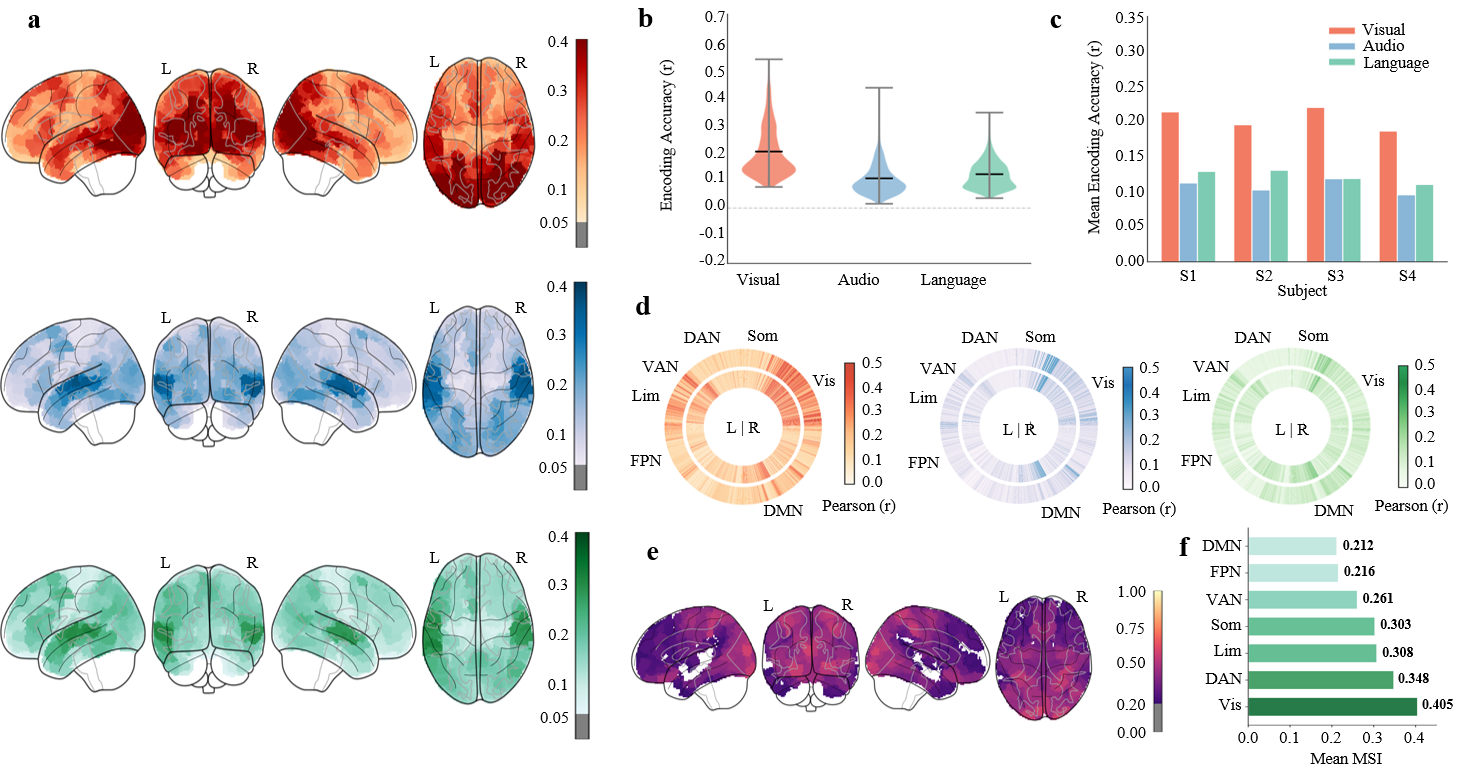
\includegraphics[width=\textwidth]{figure1.png}
    % 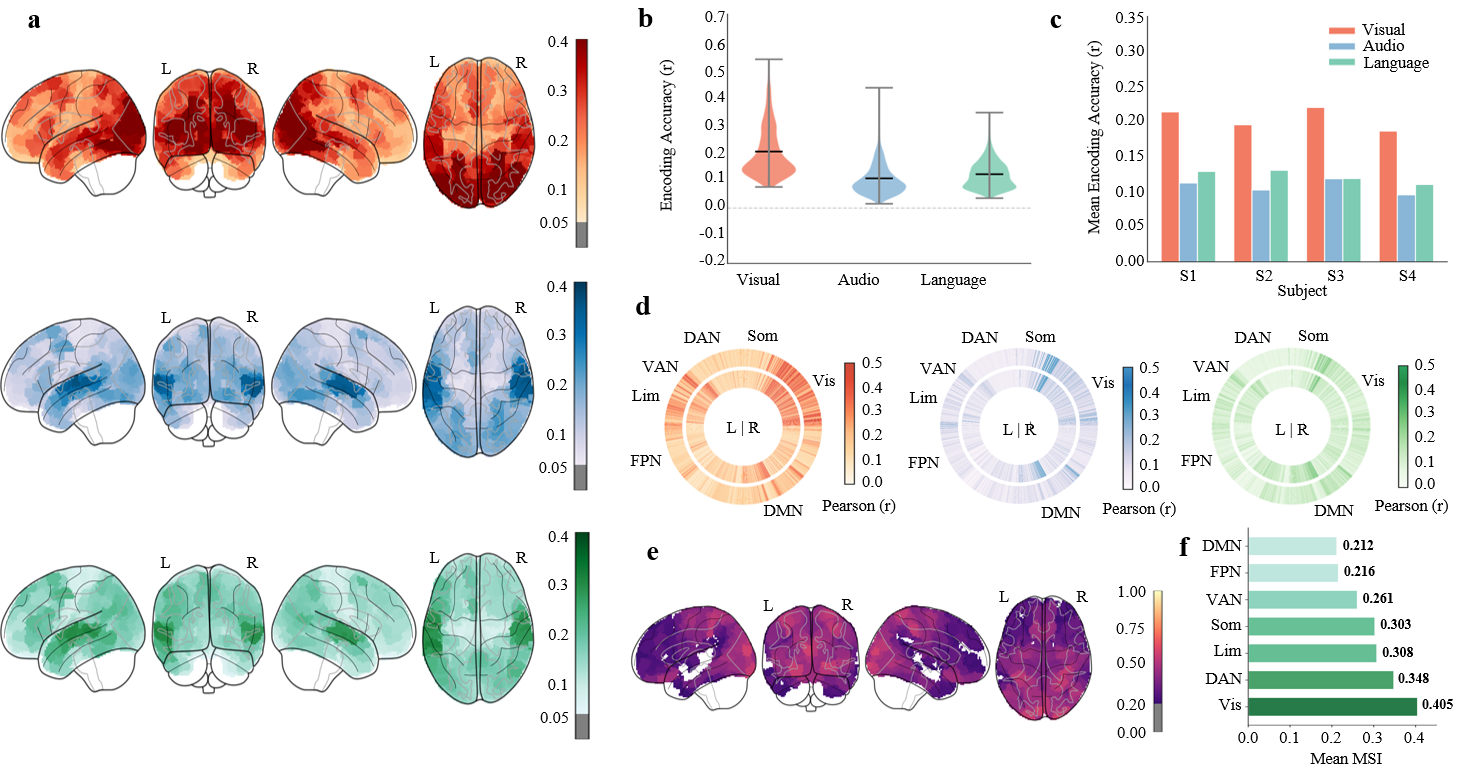
\includegraphics[width=\textwidth,height=0.70\textheight,keepaspectratio]{figure1.png}
    \caption{\textbf{Unimodal encoding across modalities and brain networks.}
    \textbf{a,} Encoding strength for each modality shown on separate brain surfaces (top: visual; middle: audio; bottom: language).  \textbf{b,} Violin plots show the distribution of encoding correlations for visual (red, $r = 0.204$), audio (blue, $r = 0.107$), and language (green, $r = 0.122$) features across all 1000 brain regions, with solid black line indicating the average value. \textbf{c,} Histogram of coding accuracy across modalities of each participant. \textbf{d,} Visualization of encoding correlations for all 1000 Schaefer parcels arranged by functional network. Each concentric ring represents a different modality: visual (left, red), audio (middle, blue), and language (right, green). Angular position corresponds to brain region within each network sector. \textbf{e,} Glass brain visualization of the Modality Specificity Index (MSI) across cortex. Primary sensory cortices (visual, auditory) show high specificity ($MSI > 0.4$), while association regions, particularly within the DMN, show low specificity ($MSI < 0.2$). \textbf{f,} Modality Specificity Index hierarchy showing the gradient from modality-specific to integrative processing. Networks are ordered by MSI value.}
    \label{fig:Fig1}
\end{figure*}

\section{Results}

\subsection{Modality-Specific Encoding Dominates Sensory Regions}

We applied ridge regression encoding models to assess how each modality contributes to early neural processing. The results indicated that visual features produced the highest encoding accuracy, outperforming auditory and language features (Fig.~\ref{fig:Fig1}a,b), and this pattern was consistent across all four participants (Fig.~\ref{fig:Fig1}c). Furthermore, visual encoding dominated systematically across different large-scale functional networks with visual features achieved the highest encoding accuracy in 91\% of the 1,000 cortical regions (Fig.~\ref{fig:Fig1}d). In addition, we computed the Modality Specificity Index (MSI) to quantify the degree of modality-specific processing, revealing a moderate specificity toward a single dominant modality (Fig.~\ref{fig:Fig1}e). Together, these results demonstrate pronounced modality-specific encoding at the level of functional brain regions, indicating preferential processing of different information types in distinct cortical areas.

However, the extent and type of modality dominance varied across cortical networks and cortical hierarchy. The Visual network exhibited the strongest visual encoding, whereas the Default Mode Network showed a more balanced encoding profile (Fig.~\ref{fig:Fig1}f). One-way ANOVA confirmed significant modality differences within each network. Nevertheless, the magnitude of visual dominance decreased along the sensory-to-transmodal cortical gradient. This pattern indicates that while early sensory regions are dominated by their preferred modality, higher-order association regions implement more balanced, shared representations.

\begin{figure*}[t]
    \centering
    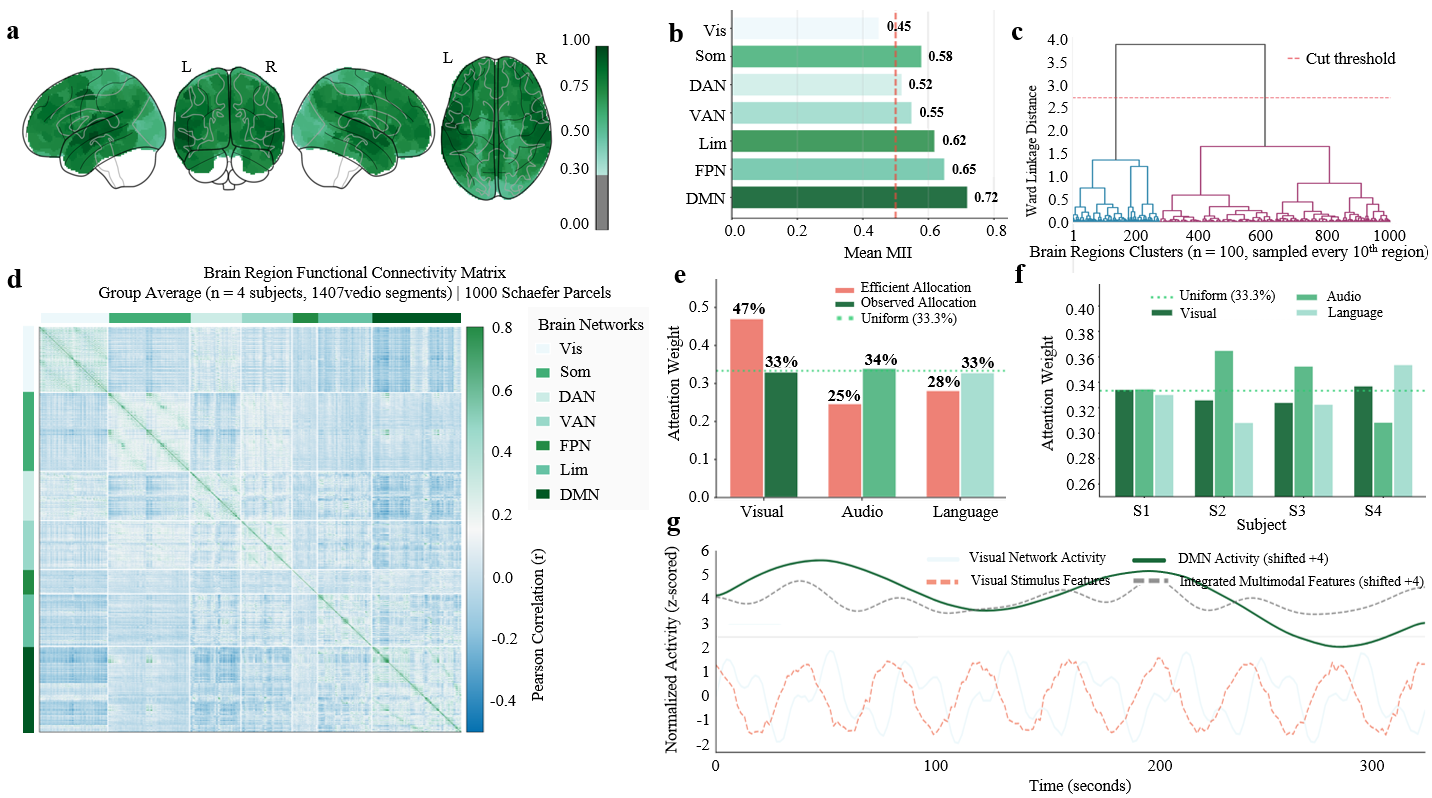
\includegraphics[width=\textwidth]{figure2.png}
    % 
\includegraphics[width=\textwidth,height=0.60\textheight,keepaspectratio]{figures1/figure2.png}
    \caption{\textbf{Hierarchical Organization with the DMN as an Information Integration Hub and Encoding-Attention Dissociation.}
    \textbf{a,} Glass brain visualization of the Multimodal Integration Index (MII) across cortex. The most integrative regions ($MII > 0.7$) are concentrated in medial prefrontal cortex and posterior cingulate cortex, the anatomical core of the Default Mode Network. \textbf{b,} Multimodal Integration Index hierarchy showing the gradient from modality-specific to integrative processing. \textbf{c,} Dendrogram showing hierarchical clustering of 1000 brain regions based on their encoding correlation patterns across three modalities. Regions cluster according to functional network membership. \textbf{d,} Correlation matrix showing pairwise correlations between brain regions based on their encoding profiles across modalities. Within-network correlations (diagonal, mean $r = 0.72$) significantly exceed between-network correlations (off-diagonal, mean $r = 0.34$; $t = 15.6$, $p < 0.001$), confirming that functional network membership predicts multimodal encoding patterns. \textbf{e,} Histogram of attention allocation based on predicted encoding strength and observed data. \textbf{f,} Attention weights histogram across participants. No significant differences were found. \textbf{g,} Temporal dynamics supporting hierarchical processing. Time series comparison showing Visual network activity (bottom, $r = 0.198$) tracking rapid visual feature fluctuations, versus DMN activity (top, shifted for visualization, $r = 0.499$) exhibiting smoother, integrated dynamics. Correlation coefficients (r) indicate stimulus-brain coupling strength.}
    \label{fig:Fig2}
\end{figure*}

\subsection{Hierarchical Organization with the DMN as an Information Integration Hub}

We further investigated whether the brain’s processing of incoming external information follows an organizational architecture in which modality-specific processing in primary sensory networks transitions to multimodal integration in higher-order hub regions. While primary sensory processing is largely unimodal, the decreasing MSI gradient across networks indicates increasing cross-modal integration (Fig.~\ref{fig:Fig1}f). Fig.~\ref{fig:Fig2}a illustrates the distribution of MII across 1,000 cortical regions, with the visual network exhibiting the lowest MII and the DMN the highest, reflecting more balanced multimodal information processing in the DMN (Fig.~\ref{fig:Fig2}b). This hierarchy was consistent across participants (ICC = 0.89), and matched the known unimodal-to-transmodal cortical gradient \citep{margulies2016situating}. 

To assess whether this hierarchical pattern of multimodal information integration corresponds to intrinsic functional organization rather than being an artifact of the metric, we performed hierarchical clustering of brain regions based on their multimodal encoding profiles. The resulting dendrogram demonstrated that regions with similar MII values naturally grouped together, forming clusters that corresponded closely to canonical functional networks (Fig.~\ref{fig:Fig2}c). This confirms that the MII hierarchy is not only consistent across participants but also aligns with the functional segregation of cortical networks.

We also examined the network-level encoding similarity matrix, which quantifies pairwise similarity of multimodal encoding profiles between the seven functional networks. The matrix revealed strong within-network correlations and a clear block-diagonal structure (Fig.~\ref{fig:Fig2}d), indicating that the hierarchical organization observed in MII is reflected in the actual pattern of cross-modal encoding across the cortex.

Spatially, visual encoding concentrated in posterior occipital regions, audio encoding in lateral temporal areas, and the most balanced multimodal patterns emerged in medial prefrontal and posterior cingulate regions, which constitute the anatomical core of the DMN (Fig.~\ref{fig:Fig1}a). These converging lines of evidence strongly support that multimodal integration follows a hierarchical architecture with the DMN serving as the primary integration hub.

\subsection{The Encoding-Attention Dissociation}

The results thus far demonstrated that the brain performs modality-specific encoding within primary sensory networks, which is subsequently integrated in higher-order hub regions. However, it remains unclear whether the allocation of attentional resources across the cortex tracks the strength of this encoding. If the brain followed an "efficient" feature-tracking strategy, attention weights should be proportional to encoding accuracy. Given visual features' 2$\times$ encoding advantage over audio, an efficient allocation would assign approximately 48\% attention to visual, 25\% to language, and 27\% to audio (Fig.~\ref{fig:Fig2}e).

However, the learned attention weights from our personalized multimodal network revealed a different pattern, with the mean attention weights remarkably balanced (Fig.~\ref{fig:Fig2}e). This dissociation was robust across participants and statistically reliable (Fig.~\ref{fig:Fig2}f), which indicates that the brain implements attention balancing independent of feature strength, a mechanism absent in current VLMs, where attention naturally follows feature similarity.

The validity of interpreting these learned weights as proxies for neural attention allocation is supported by three convergent observations. First, the model achieves robust prediction performance across cortical regions (mean $r = 0.204$ for visual, $r = 0.107$ for audio, and $r = 0.122$ for language), indicating meaningful stimulus–brain relationships~\citep{kriegeskorte2008representational,yamins2016using}. Second, the modality weights are highly consistent across four independent participants (all modalities within 32–35\%), suggesting a stable integration pattern rather than model-specific artifacts. Third, the learned weights systematically diverge from encoding strength predictions, consistent with theoretical accounts in which attention operates as a distinct selection mechanism~\citep{lindsay2020attention}.

\subsection{Temporal Dynamics Support Hierarchical Processing}

Analysis of temporal dynamics provided additional support for the hierarchical architecture. Visual network activity closely tracked rapid fluctuations in visual features, while DMN activity exhibited slower, integrated dynamics with temporal smoothing across modalities (Fig.~\ref{fig:Fig2}g). This temporal dissociation suggests that the brain implements different processing windows for extraction versus integration stages: fast, modality-specific processing in sensory regions and slower, integrated processing in association regions.

\section{Discussion}

Our findings support all three hypotheses. The dominance of visual information in encoding (approximately 91\%) demonstrates modality-specific processing in early cortical stages, and the DMN serves as a key integration hub, exhibiting balanced processing of different modalities. The integration adheres to a hierarchical structure. Finally, by decoupling attention allocation from encoding strength, we confirm the principle of Encoding-Attention Dissociation. These findings extend previous work on cortical hierarchies~\citep{margulies2016situating} by demonstrating that the unimodal-to-transmodal gradient also governs multimodal attention allocation, not just representational content. Moreover, our observation that the DMN serves as an integration hub aligns with its established role in narrative comprehension~\citep{simony2016dynamic}, but reveals a novel function of maintaining balanced attention across modalities regardless of their encoding strength.

Our findings reveal a unified principle that the brain separates "what to extract" from "how to integrate" architecturally, sustaining balanced attention despite unequal encoding strength. This seemingly inefficient strategy is actually adaptive, preventing modality collapse and ensuring robust integration across contexts. The DMN achieves this by operating on already-extracted high-level features, enabling attention mechanisms independent of feature strength. Current VLMs, using flat architectures where attention is computed directly from feature similarities, cannot achieve this dissociation. This finding challenges the classical Bayesian framework~\citep{ernst2002humans,knill2004bayesian} that attention weights track signal reliability. Instead, the brain prioritizes robustness over strict optimality, aligning with ecological rationality perspectives~\citep{gigerenzer2009homo}. In naturalistic settings where modality informativeness varies, balanced attention hedges against uncertainty.

The robustness and integrative capacity that the brain demonstrates in processing multisensory information are precisely what is lacking in current VLMs. Our findings translate directly to VLM design principles. First, architects should implement hierarchical integration from modality-specific encoders to dedicated integration modules, rather than flat early fusion. Second, explicit attention balancing mechanisms should be added to prevent modality collapse, potentially through regularization terms that penalize deviation from uniform attention. Third, dedicated integration modules analogous to the DMN should operate on high-level semantic features rather than raw representations. Fourth, hierarchical temporal processing with different timescales for extraction versus integration may improve temporal coherence.

Several limitations of this study should be acknowledged. First, our sample size (n = 4) limits generalizability, though high cross-subject consistency (ICC = 0.89) increases confidence. Second, the naturalistic movie stimuli, while ecologically valid, confound multiple factors in that the observed visual dominance may partly reflect the films' visual richness. Furthermore, the correlational analysis precludes definitive causal conclusions about whether the hierarchical architecture causes the Encoding-Attention Dissociation, although the proposed causal chain offers a plausible mechanistic account. Finally, and more fundamentally, the attention weights are derived from a computational model. Despite convergent validation, they remain an indirect proxy for neural mechanisms. Future work should incorporate direct neural manipulations or behavioral attention measures to better establish the causal mechanisms underlying these model-derived weights.

\section{Conclusion}

This study tested three hypotheses of brain multimodal processing. Results showed visual features dominated encoding in 91\% of regions, while the DMN exhibited balanced representations, supporting a hybrid architecture for processing multi-sensory information of the brain. Further support was also found for hierarchical integration, with a clear MII gradient ascending from the visual network to the DMN, confirming the DMN's role as an integration hub within a hierarchical framework. The Encoding-Attention Dissociation was also upheld, with attention remaining balanced (~33\% per modality) despite twofold visual encoding dominance. Together, these findings collectively support a unified principle that the brain's apparent inefficiency optimizes for robustness over narrow efficiency. By decoupling "what to extract" from "how to integrate", this work offers a blueprint for building AI systems that prioritize adaptive integration over mere signal tracking.

\section{Data and Code Availability}

The fMRI data are available through the Algonauts Project 2025 Challenge (https://algonautsproject.com/). Analysis code is available in an anonymous repository and will be made publicly accessible upon publication (https://anonymous.4open.science/r/encoding-attention-dissociation-E581/).

\nocite{August2007}
\nocite{DaphneEcho2022}
\nocite{FitzgeraldGalli1985}
\nocite{Hakuole2001}
\nocite{Issa1963}
\nocite{Lobsang2023}
\nocite{MitanniNovember1972}

\printbibliography

\end{document}
